\section{ALGORITHM\textbackslash METHODOLOGY}

\subsection{Algorithm}
\noindent\uline{Five types of Platonic Solids}: 
\begin{figure}[h]
\centering
	\includegraphics[width=1\textwidth]{image/rollingDir2.pdf}
	\caption{Rolling direction for each types of platonic solids}
	\label{fig:platonicSolids}
\end{figure}\\
%
% 
%
%
%
%
%
\uline{Version1}: \\


Example:\\
\begin{algorithm}[H]
\SetAlgoLined
\KwResult{\textit{Write here the result }}
 initialization\;
 \While{While condition}{
  instructions\;
  \eIf{condition}{
   instructions1\;
   instructions2\;
   }{
   instructions3\;
  }
 }
 \caption{How to write algorithms}
\end{algorithm}


\noindent\uline{Version2}: 
% algorithm code (for this example)
\begin{algorithm}

% functions
\SetKwFunction{cumprod}{cumprod}
\SetKwFunction{length}{length}
\SetKwFunction{zeros}{zeros}
\SetKwFunction{ceil}{ceil}

% input/ouput names
\SetKwInOut{Input}{Input}
\SetKwInOut{Output}{Output}

% caption
\caption{Creation of edge set for a specific perfect matching number.\label{alg:singlepm}}

\Input{%
		\xvbox{2mm}{$\xvar{N}$} -- number of vertices (should be even) \\
		\xvbox{2mm}{$\xvar{I}$} -- perfect matching number, integer between 1 and $(\xvar{N}-1)!!$
	  }
\Output{%
		\xvbox{2mm}{$\xvar{E}$} -- vector of edges in sequential pairs
	   }

  \BlankLine % blank line for spacing
  
  % start of the pseudocode
  \xvbox{2mm}{$\xvar{J}$} $\leftarrow$ $[ 1,3,5,\dots,\xvar{N}-1 ]$ \tcc*{odd numbers from 1 to N-1}

  \xvbox{2mm}{$\xvar{P}$} $\leftarrow$ $[ 1,\cumprod(\xvar{J}) ]$ \tcc*{cumulative double factorial}
    
  \xvbox{2mm}{$\xvar{V}$} $\leftarrow$ $[ 1,2,\dots,\xvar{N} ]$ \tcc*{create initial list of available vertices}
        
  \For{$\xvar{j}\leftarrow$ $\xvar{J}$ }{

    \xvbox{1mm}{$\xvar{q}$} $\leftarrow$ $(\xvar{N}+1-\xvar{j})/2$ \tcc*{index for 2nd to last entry in P}

    \xvbox{1mm}{$\xvar{I}$} $\leftarrow$ $\ceil\big(\xvar{I}/\xvar{P}(\xvar{q})\big)$ \tcc*{calculate smaller vertex index}

    $\xvar{E}(\xvar{j})$ $\leftarrow$ $\xvar{V}(\xvar{end})$ \tcc*{assign largest remaining value}

    remove element $\xvar{V}(\xvar{end})$ \tcc*{remove largest remaining value}

    $\xvar{E}(\xvar{j}+1)$ $\leftarrow$ $\xvar{V}(\xvar{i})$ \tcc*{assign smaller selected value}

    remove element $\xvar{V}(\xvar{i})$ \tcc*{remove the smaller selected value}

    \xvbox{1mm}{$\xvar{I}$} $\leftarrow$ $\xvar{I} - \big( (\xvar{i} - 1) \times \xvar{P} (\xvar{q}) \big)$ \tcc*{subtract to get index in subgraph with 2 vertices removed}
	
  } % end for j	

\end{algorithm}


\clearpage
\newpage

%----------------------------------
\subsection{Nodes}
%\begin{figure}
	\tikzset{
	level/.style={sibling distance=35mm/#1},
	treenode/.style={align=center,inner sep=0pt},
	% Black nodes
	node_black/.style={treenode,circle,black,draw=black,very thick,text width=0.5cm},
	% Red nodes
	node_red/.style={treenode,circle,red,draw=red,very thick,text width=0.5cm},
	% Blue nodes
	node_blue/.style={treenode,circle,blue,draw=blue,very thick,text width=0.5cm},
	% Nil nodes
	node_nil/.style={treenode,rectangle,fill=black,minimum width=0.3cm,minimum height=0.3cm}
}
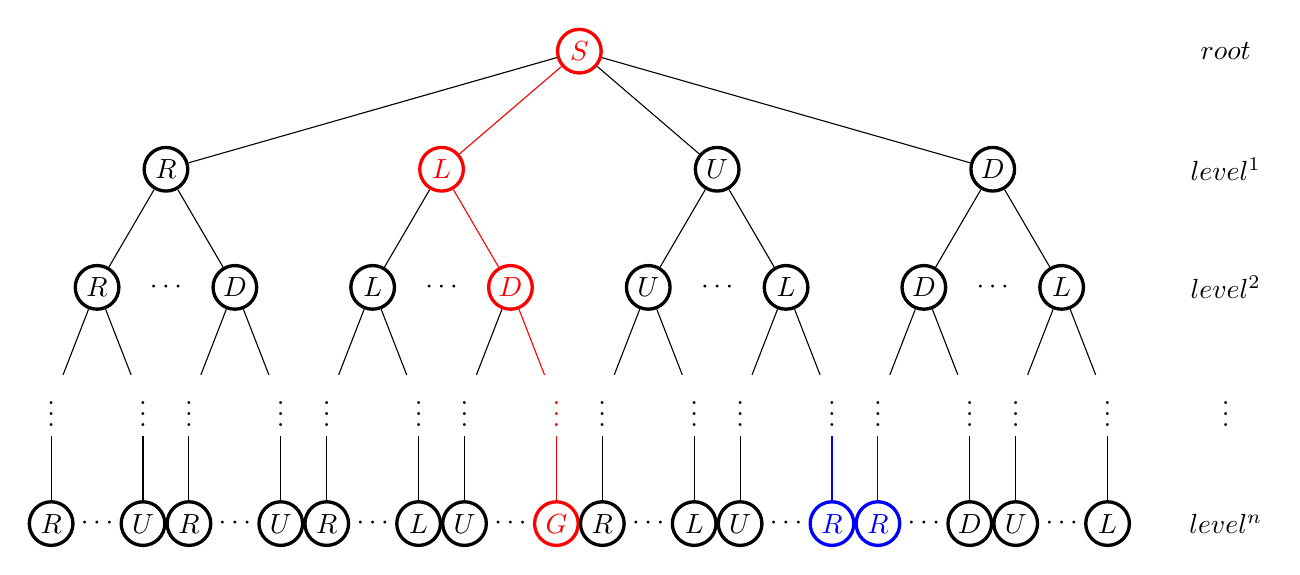
\begin{tikzpicture}

\node[node_red] (z){$S$}
  child {node[node_black] (a) {$R$}								%%% Right
    child[black] {node[node_black]  (b) {$R$}
      child {node (b1) {$\vdots$}
       child {node[node_black] (b11) {$R$}}
      }
      child {node (b2) {$\vdots$}
       child {node[node_black] (b12) {$U$}}
      }
    }
    child[black] {node[node_black] (g) {$D$}
      child {node (g1) {$\vdots$}
       child {node[node_black] (g11) {$R$}}
      }
      child {node (g2) {$\vdots$}
       child {node[node_black] (g12) {$U$}}
      }
    }
  }
   child[red] {node[node_red] (d) {$L$}                    %%%% LEft - the shortest parth
      child[black] {node[node_black]  (e) {$L$}
        child {node (e1) {$\vdots$}
         child {node[node_black] (e11) {$R$}}
        }
        child {node (e2) {$\vdots$}
         child {node[node_black] (e12) {$L$}}
        }
      }
      child[red] {node[node_red] (f) {$D$}
        child[black] {node (f1) {$\vdots$}
         child[black] {node[node_black] (f11) {$U$}}
        }
        child[red] {node (f2) {$\vdots$}
         child[red] {node[node_red] (f12) {$G$}}
        }
      }
    }
    child[black] {node[node_black] (m) {$U$}      %%% Up
      child {node[node_black]  (n) {$U$}
        child {node (n1) {$\vdots$}
         child {node[node_black] (n11) {$R$}}
        }
        child {node (n2) {$\vdots$}
         child {node[node_black] (n12) {$L$}}
        }
      }
      child {node[node_black] (o) {$L$}
        child {node (o1) {$\vdots$}
         child {node[node_black] (o11) {$U$}}
        }
        child {node (o2) {$\vdots$}
         child[blue] {node[node_blue] (o12) {$R$}}
        }
      }
    }
  child[black] {node[node_black]  (j) {$D$}   %%% Down
    child {node[node_black] (k) {$D$}
      child {node {$\vdots$}
       child[blue] {node[node_blue] (k11) {$R$}}
      }
      child {node {$\vdots$}
       child {node[node_black] (k12) {$D$}}
      }
    }
    child {node[node_black] (l) {$L$}
    child {node {$\vdots$}
     child {node[node_black] (l11) {$U$}}
    }
    child {node (c){$\vdots$}
     child {node[node_black] (l12) {$L$}
            child [grow=right] {node (r) {$level^n$} edge from parent[draw=none]
              child [grow=up] {node (s) {$\vdots$} edge from parent[draw=none]
                child [grow=up] {node (t) {$level^2$} edge from parent[draw=none]
                  child [grow=up] {node (u) {$level^1$} edge from parent[draw=none]
                   child [grow=up] {node (u) {$root$} edge from parent[draw=none]}
                                   }
                                 }
                               }
                               }
            }
          }
         }
};
\path (b) -- (g) node [midway] {$\cdots$};\path (n) -- (o) node [midway] {$\cdots$};
\path (e) -- (f) node [midway] {$\cdots$};
\path (k) -- (l) node [midway] {$\cdots$};
\path (b11) -- (b12) node [midway] {$\cdots$};
\path (g11) -- (g12) node [midway] {$\cdots$};\path (n11) -- (n12) node [midway] {$\cdots$};
\path (e11) -- (e12) node [midway] {$\cdots$};\path (o11) -- (o12) node [midway] {$\cdots$};
\path (f11) -- (f12) node [midway] {$\cdots$};
\path (k11) -- (k12) node [midway] {$\cdots$};
\path (l11) -- (l12) node [midway] {$\cdots$};

%\begin{tikzlegend}[legend entries={monopolist profit within entry allowance,
%      monopolist profit within entry deterrence,something else},
%        legend style={at={(0,-1)},anchor=north west}, legend cell align=left]
%     \addlegendimage{dotted,sharp plot}
%     \addlegendimage{sharp plot}
%     \addlegendimage{dashed, sharp plot}
%\end{tikzlegend}   
   
\end{tikzpicture}

%% take notes

\vskip 0.5cm

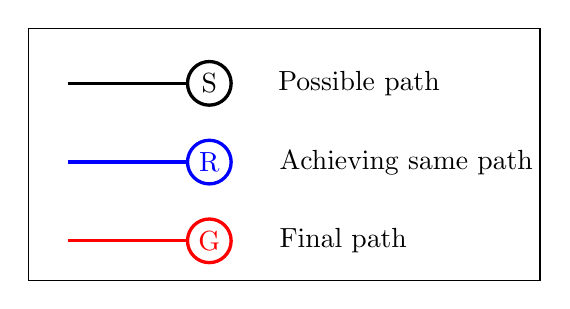
\begin{tikzpicture}
\draw (-0.5,-2.5) rectangle(6,0.7);
\draw[-][draw=black, very thick] (0,0) -- (1.5,0);
\draw (1.8,0) node[node_black]{S}  ;
\draw (3.7,0) node{Possible path} ;
\draw[-][draw=blue, very thick] (0,-1) -- (1.5,-1);
\draw (1.8,-1) node[node_blue]{R} ;
\draw (4.3,-1) node{Achieving same path} ;
\draw[-][draw=red, very thick] (0,-2) -- (1.5,-2);
\draw (1.8,-2) node[node_red]{G} ;
\draw (3.5,-2) node{Final path} ;
\end{tikzpicture}
%\vskip 0.5cm
%\end{figure}

%----------------------------------
\clearpage
\newpage